\documentclass[
  accentcolor=tud1c,	% Color theme for TUD corporate design
  colorbacktitle,		% Titlepage has colored background for title area
  inverttitle,			% Font color of title on titlepage is inverted
  german,				% Document is in english
  twoside
]{tudexercise}

\usepackage[ngerman]{babel}
\usepackage{units}
\usepackage{hyperref}
\usepackage[utf8]{inputenc}


\definecolor{commentgreen}{RGB}{50,127,50}


\usepackage{listings}
\usepackage{listings}
\lstloadlanguages{C++}
\lstset{language=C++}
\lstset{captionpos=b}
\lstset{tabsize=3}
\lstset{breaklines=true}
\lstset{columns=flexible,keywordstyle=\color{purple},stringstyle=\color{blue},commentstyle=\color{commentgreen}}
\lstset{literate=%
{Ö}{{\"O}}1
{Ä}{{\"A}}1
{Ü}{{\"U}}1
{ß}{{\ss}}2
{ü}{{\"u}}1
{ä}{{\"a}}1
{ö}{{\"o}}1
{'}{{\textquotesingle}}1
}

\parindent0pt

\newcommand{\tag}{2}

\title{Übung zum\linebreak[1]C/C++-Praktikum\linebreak[1] Fachgebiet Echtzeitsysteme}
\subtitle{Übungen für den \tag{}. Tag}

\begin{document}

\begin{examheader}
	\textmb{Übung zum C/C++-Praktikum - Tag \tag{}}
\end{examheader}
\maketitle 

\vspace{5mm}

\section{Zeiger und Referenzen Grundlagen}

\begin{enumerate}

\item Experimentieren Sie mit Zeigern, Adressen und Referenzen. Versuchen Sie ein Bild ähnlich wie im Skript zu zeichnen, dass Ihnen verdeutlicht, wie Variablen und ihre Speicherabbilder zusammenhängen. Als Ausgangsbasis kann dieses Programmfragment dienen:
\begin{lstlisting}
int intVal = 42;
int* pIntVal = &intVal;
cout << "Wert von IntVal " << intVal << endl;
cout << "Wert von &IntVal " << &intVal << endl;
cout << "Wert von pIntVal " << pIntVal << endl;
cout << "Wert von *pIntVal " << *pIntVal << endl;
cout << "Wert von &pIntVal " << &pIntVal << endl;
\end{lstlisting}

\item Seien \emph{intVal} und \emph{pIntVal} wie oben gegeben. Versuchen Sie die Bedeutung folgender Ausdrücke zu verstehen. Tipp: gehen Sie dabei von innen nach außen vor.

\begin{lstlisting}
*&intVal;
\end{lstlisting}

\begin{lstlisting}
*&pIntVal;
\end{lstlisting}

\begin{lstlisting}
&*pIntVal;
\end{lstlisting}

\begin{lstlisting}
**&pIntVal;
\end{lstlisting}

\begin{lstlisting}
*&*&intVal;
\end{lstlisting}

\begin{lstlisting}
&*&pIntVal;
\end{lstlisting}

\begin{lstlisting}
*&*pIntVal;
\end{lstlisting}


\item Versuchen Sie zu verstehen, warum folgende Ausdrücke ungültig sind. Tipp 1: Finden Sie heraus, welchen Typ der Ausdruck hätte haben müssen. Tipp 2: Nur tatsächlich angelegte Variablen haben Adressen. Ausdrücke wie a + b oder direkt kodierte Zahlenliterale wie 42 haben keine Adresse.

\begin{lstlisting}
*intVal;
\end{lstlisting}

\begin{lstlisting}
**pIntVal;
\end{lstlisting}

\begin{lstlisting}
**&*pIntVal;
\end{lstlisting}

\begin{lstlisting}
&*intVal;
\end{lstlisting}

\begin{lstlisting}
&42;
\end{lstlisting}

\item Schreiben Sie eine Funktion, die zwei int-Variablen miteinander vertauscht. Probieren Sie dabei beide möglichen Übergabevarianten (by-Reference, by-Pointer) aus. 

\item Folgendes Programm sei gegeben:\\

\begin{minipage}{\textwidth}
\begin{lstlisting}
void foo(int& i) {
	int i2 = i;
	int& i3 = i;
	
	cout << "i = " << i << endl;
	cout << "i2 = " << i2 << endl;
	cout << "i3 = " << i3 << endl;
	cout << "&i = " << &i << endl;
	cout << "&i2 = " << &i2 << endl;
	cout << "&i3 = " << &i3 << endl;
}

int main() {
	int var = 42;
	cout << "&var = " << &var << endl;
	foo(var);
}
\end{lstlisting}
\end{minipage}

Welche Adressen werden übereinstimmen, welche werden sich unterscheiden? Probieren Sie das Programm aus und versuche Sie, die Ausgabe nachzuvollziehen.

\end{enumerate}

\section{Arrays und Zeigerarithmetik}
Arrays sind zusammenhängende Speicherbereiche, die mehrere Variablen von gleichem Typ speichern können. Arrays werden in C++ folgendermaßen angelegt:

\begin{lstlisting}
	<Typ> <name>[<Größe>];
\end{lstlisting}

z.B.
\begin{lstlisting}
	int arr[10]; // array of 10 integers
\end{lstlisting}

Falls das Array global ist, muss die Größe eine konstante Zahl sein, falls das Array in einer Funktion auf dem Stack angelegt wurde, kann die Größe auch durch eine Variable vorgegeben werden. Auf jeden Fall bleibt diese während der Existenz des Arrays konstant und kann sich nach dem Anlegen nicht mehr ändern.\\
Beim anlegen eines Arrays kann man dieses auch direkt initialisieren:
\begin{lstlisting}
	int arr[5] = { 1 , 2, 3, 4, 5};
\end{lstlisting}
Man kann die Größe optional auch weglassen, in diesem Fall wird sie der Compiler anhand der angegebenen Elemente selbst ermitteln. \\

Man kann auf die einzelnen Elemente des Arrays wie gewohnt über 
\textbf{arr[i]}
zugreifen. \\

Arrays und Zeiger sind in C++ stark miteinander verwandt. So ist der \textbf{Bezeichner} des Arrays gleichzeitig die \textbf{Adresse des ersten Elements}. Somit kann man sowohl durch \textbf{*arr} als auch durch \textbf{arr[0]} auf das erste Element zugreifen.
Analog dazu kann man auch einen Zeiger auf das erste Element anlegen:
\begin{lstlisting}
	int* pArr = arr;
\end{lstlisting}
Da die Elemente eines Array direkt hintereinander stehen, kann man den Zeiger inkrementieren, um zum  nächsten Element zu gelangen. Beispiel:

\begin{lstlisting}
	int* pArr = arr;
	cout << "Adresse des ersten Elements: " << pArr << endl;
	cout << "Adresse des zweiten Elements: " << pArr+1 << endl;
	cout << "Adresse des dritten Elements: " << pArr+2 << endl;
\end{lstlisting}

Somit kann man auf beliebige Elemente des Array über den Zeiger zugreifen:
\begin{lstlisting}
	*(pArr+0); // erstes Element
	*(pArr+1); // zweites Element
	*(pArr+2) // drittes Element
	*(pArr + i) // i-tes Element
	
	pArr++; // inkrementiere Zeiger im 1 !!!
	
	*(pArr + 0) // ZWEITES Element von arr
	*(pArr + 2) // VIERTES Element von arr
\end{lstlisting}

Tatsächlich ist \textbf{*(p+i)} in \textbf{jeder Hinsicht äquivalent} zu \textbf{p[i]}. Das bedeutet, dass man sowohl auf das i-te Element eines Arrays über \textbf{*(arr + i)} zugreifen kann, als auch über \textbf{pointer[i]} auf das Element, auf welches der Zeiger \emph{pointer+i} zeigt!

\begin{enumerate}
\item Legen Sie in der main-Funktion ein int-Array mit 10 Elementen an, und initialisieren Sie es mit den Zahlen 1 bis 10. Iterieren Sie in einer Schleife über das Array und geben Sie alle Elemente nacheinander aus.

\item In C++ kann man Arrays nicht direkt an Funktionen übergeben. Stattdessen übergibt man einen Zeiger auf das erste Element des Arrays. Aufgrund der Äquivalenz von \textbf{*(p+i) } und \textbf{p[i]} kann man in der Funktion den Zeiger syntaktisch wie das Original-Array verwenden.

Schreiben Sie eine Funktion, die einen const-Zeiger auf das erste Element eines Arrays bekommt und alle Elemente ausgibt. Da die Funktion nur anhand des Zeigers keine Möglichkeit hat zu wissen, wie groß das Array ist, muss die Größe des Arrays durch einen weiteren Parameter übergeben werden. 

\item Wie wir vorher gesehen haben, kann man mit Zeigern auch rechnen und diese nachträglich ändern. Anstatt mit einem Index das Array zu durchlaufen, kann man stattdessen bei jeder Iteration den Zeiger selbst inkrementieren! 

\begin{lstlisting}
	for(int* p = pArr; p != pArr + 10; p++) {
		// *p contains current element
		...
	}
\end{lstlisting}

Schreiben Sie die Funktion aus der vorherigen Aufgabe so um, dass sie einen laufenden Zeiger anstatt eines Indices verwendet.

\item Ebenso kann man auch die Arraygröße auf eine andere Weise übergeben, indem man stattdessen die Adresse des Elements nach dem letzten Element angibt. Dadurch werden Schleifen der Form
\begin{lstlisting}
	for(int* p = begin; p != end; p++) {
		// *p contains current element
		...
	}
\end{lstlisting}

möglich. Schreiben Sie die Funktion aus der vorherigen Aufgabe entsprechend um. Vergessen Sie nicht, den Zeiger als const zu definieren, da Elemente nur gelesen werden.

\item Die obige Methode, über Elemente eines Arrays zu iterieren, mag Ihnen zunächst etwas ungewöhnlich erscheinen. Diese hat aber den Vorteil, dass man anstatt des ganzen Arrays auch nur einen (zusammenhängenden) Teil davon an Funktionen übergeben kann, indem man Zeiger auf die entsprechenden Anfangs-und Endelemente bildet. Beispiel:
\begin{lstlisting}
	int arr[10];
	printElements(arr+5, arr+8); // Print elements with index 5, 6, 7
\end{lstlisting}
Experimentieren Sie mit dieser Übergabemethode in Zusammenhang mit Ihrer bisherigen Ausgabefunktion!

\item Bisher haben wir das Array auf dem Stack angelegt. Mit \textbf{new[]} kann man ein Array auf dem Heap erzeugen. Dabei wird die Adresse des ersten Elements in einem Zeiger gespeichert. Mittels \textbf{delete[]} kann (muss!) man den belegten Speicher nach Benutzung wieder freigeben. Beispiel:
\begin{lstlisting}
	int* pArr = new int[10]; // size can be a variable
	doSomethingWith(pArr, 10);
	delete[] pArr; // <-- notice the [] !
\end{lstlisting}
Beachten Sie die \textbf{[]} nach delete. Diese geben an, dass ein Array und nicht bloß ein Element gelöscht werden soll.

Ein Anwendungsfall von dynamischen Arrays sind Funktionen, die ein Array von vorher unbekannter Größe zurückgeben. Schreiben Sie eine Funktion, die beliebig viele Zahlen von der Konsole mittels \emph{cin} einließt. Der Benutzer soll dabei zuvor gefragt werden, wie viele Zahlen er eingeben möchte. Speichern Sie die Zahlen in einem dynamisch angelegten Array ab und lassen Sie die Funktion den Zeiger darauf zurückgeben. 

Zusätzlich zum Zeiger muss die Funktion auch die Möglichkeit haben, ihrem Aufrufer die Größe des angelegten Arrays mitzuteilen. Fügen Sie der Funktion deshalb einen weiteren Parameter hinzu, in dem entweder per Referenz oder per Zeiger eine Variable übergeben wird, um dort die Größe abzulegen. 

Geben Sie die eingelesenen Werte wieder auf der Konsole aus.
Vergessen Sie nicht, am Ende den Speicher wieder freizugeben.
\end{enumerate}

Noch ein paar Worte zum Schluss: In C++ findet keine automatische Bereichsprüfung bei Arrayzugriffen statt. Sie sind als Programmierer selbst dafür verantwortlich, dass niemals auf ein Element außerhalb der Array-Grenze zugegriffen wird. Falls doch, kann es zu Programmabstürzen oder unerwünschten Effekten wie z.B. einem Buffer-Overflow kommen, der ein erhebliches Sicherheitsrisiko darstellt. Bevorzugen Sie deshalb Container-Klassen wie \emph{std::vector} aus der STL anstelle von direkten Arrays. Beachten Sie außerdem, dass der Operator \textbf{delete[]} zwar das Array löscht, den Zeiger aber \textbf{nicht} auf \emph{NULL} setzt. Dabei entsteht ein \emph{Dangling Pointer}, welcher dazu führen kann, dass später im Programm auf Speicherstellen zugegriffen wird, die nicht reserviert sind. Setzen Sie deshalb Zeiger nach einem \textbf{delete} sofort auf \emph{NULL}, um Speicherfehler zu vermeiden. \\

Um die Größe eines Arrays zu ermitteln, können Sie den \emph{sizeof()}-Operator benutzen. Dieser gibt generell die Anzahl der Bytes an, die eine Variable verbraucht. Da einzelne Array-Elemente größer als ein Byte sein können, muss die Gesamtgröße des Arrays durch die Größe eines Elements geteilt werden, um auf die Anzahl der Elemente zu kommen.
\begin{lstlisting}
	int arr[10];
	cout << sizeof(arr) << endl; // 40 on 32-bit machine, 80 on 64-bit
	int len = sizeof(arr) / sizeof(arr[0]); 
	cout << len << endl; // always 10
\end{lstlisting}

Beachten Sie, dass \emph{sizeof()} \textbf{nicht} dazu verwendet werden kann, um die Größe des Arrays herauszufinden, auf die ein Zeiger zeigt. In diesem Fall wird \emph{sizeof()} nämlich die \textbf{Größe des Zeigers} und nicht die Größe des Arrays liefern!
\begin{lstlisting}
	int arr[10];
	int* pArr = arr;
	cout << sizeof(pArr) << endl; // 4 on 32-bit machine, 8 on 64-bit
\end{lstlisting}

\section{Verkettete Listen}
In dieser Aufgabe wollen wir eine doppelt verkettete Liste von Integern implementieren. Dazu brauchen wir zwei Klassen - ein \emph{ListItem}, welches ein Element der Liste mit dem Inhalt darstellt, sowie \emph{List}, die Zeiger auf Anfangs und Endelemente enthält und den eigentlichen Zugangspunkt für die Liste bildet.

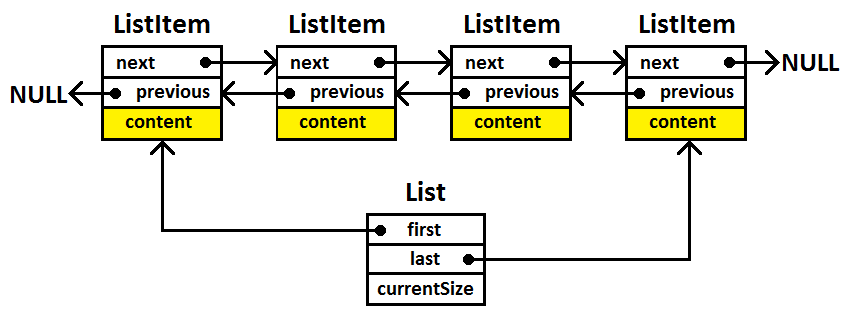
\includegraphics[width=1\textwidth]{list.png}

Wir werden am Tag 4 auf dieser Aufgabe aufbauen und die Liste um weitere Funktionen erweitern. Behalten Sie dies bitte im Hinterkopf und löschen Sie Ihre Lösung nicht. Falls Sie mit dieser Aufgabe bis dahin nicht fertig sein sollten, können Sie natürlich auch die Musterlösung als Basis nehmen.

\begin{enumerate}
\item Beginnen Sie mit der Klasse \emph{ListItem}. \emph{ListItem} soll die zu speichernde Zahl sowie Verweise auf das vorherige und nächste \emph{ListItem} als Attribute haben. Verwenden Sie dazu Zeiger und keine Referenzen, da Referenzen nachträglich nicht mehr geändert werden können. Auch können Referenzen nicht \emph{NULL} sein, was aber in unserem Fall nötig ist, um zu markieren, dass ein Element keine Vor- oder Nachfolger hat. \\

Der Konstruktor sollte sowohl seine eigenen \emph{next} und \emph{previous} Zeiger initialisieren, als auch die seiner Vor- und Nachfolgerelemente. \emph{getContent()} soll eine Referenz auf den Inhalt zurückgeben, damit dieser durch eine Zuweisung modifiziert werden kann.

\begin{lstlisting}
class ListItem {
public:
	/** 
	 * Create a list item between two elements with given content 
	 * Also modify the corresponding previous and next pointers of prev and next item
	 **/
	ListItem(ListItem* prev, ListItem* next, int content);

	/** 
	 * Delete a list item. Change also the pointers of previous and next elements to not
	 * show on this item anymore.
	**/
	~ListItem();

	/** return element content as reference */
	int& getContent();

	/** next list item, NULL if there is no next */
	ListItem* getNext();

	/** previous list item, NULL if there is no previous */
	ListItem* getPrevious();

private:
	/** previous and next items in list */
	ListItem* previous, *next;

	/** content of the list item */
	int content;
};
\end{lstlisting}

\item Unsere \emph{ListItem} Klasse hat einen kleinen Design-Fehler: da der Copy-Konstruktor nicht definiert wurde, hat der Compiler automatisch einen erzeugt. Dieser kopiert einfach die einzelnen Attribute des Ursprungsobjekts (Shallow Copy). In unserem Fall ergibt das Kopieren eines Items jedoch semantisch keinen Sinn, weil dabei ein hängendes \emph{ListItem} entstehen würde, welches nicht mit der Liste verknüpft ist, aber dennoch auf andere Items der Liste zeigt. 

Deshalb werden wir das Kopieren von \emph{ListItem}-Objekten verbieten, indem wir einen Copy-Konstruktor erstellen und diesen als private definieren. Dadurch wird es an keiner Stelle erlaubt sein, diesen aufzurufen, und der Compiler wird bei einem Versuch eine Fehlermeldung ausgeben. \\

Implementieren Sie einen leeren privaten Copy-Konstruktor
\begin{lstlisting}
	/** Copy constructor in private area to forbid copying */
	ListItem(const ListItem& other);
\end{lstlisting}

\item Implementieren Sie nun die Klasse \emph{List}. Achten Sie bei den Methoden zum Einfügen und Entfernen von Elementen darauf, dass bei einer leeren Liste eventuell sowohl die \emph{first} als auch \emph{last} Zeiger modifiziert werden müssen. Vergessen Sie außerdem nicht, \emph{currentSize} bei jeder Operation entsprechend anzupassen. Falls die Liste leer ist, sollten \emph{deleteFirst()} und \emph{deleteLast()} einfach nichts ändern.
\begin{lstlisting}
class List {
public:
	/** Create an empty list */
	List();

	/** Delete the list and all elements */
	~List();
	
	/** Create List as copy of other list */
	List(const List& other);

	/** append an element to end of the list */
	void appendElement(int i);

	/** prepend an element to beginning of the list.  */
	void prependElement(int i);
	
	/** insert element at position pos. append/prepend element if pos outside of range*/
	void insertElementAt(int i, int pos);

	/** number of elements in list */
	int getSize() const;

	/* return n-th element. No range checks. slow! */
	int& getNthElement(int n);

	/** return first element */
	int& getFirst();

	/** return last element */
	int& getLast();

	/** delete first element and return it. If list was empty, return 0. */
	int deleteFirst();

	/** delete last element and return it. If list was empty, return 0. */
	int deleteLast();
	
	/** delete element at given position. delete first/last if pos outside of range */
	int deleteAt(int pos);

private:
	/** first and last item pointers. NULL if list is empty */
	ListItem* first, *last;
	
	/** current size of the list */
	int currentSize;
};
\end{lstlisting}

\item Testen Sie Ihre Implementierung. Fügen Sie der Liste Elemente von beiden Seiten hinzu und löschen Sie auch wieder welche. Kopieren Sie die Liste und geben Sie die Elemente nacheinander aus.

\item Bisher haben wir über \emph{getNthElement()} auf die Elemente der Liste zugegriffen. Diese Methode kann insbesondere bei langen Listen sehr langsam sein. Deshalb werden wir einen Iterator schreiben, über den man auf die Listenelemente sequenziell zugreifen kann. Der Iterator soll dabei einen Zeiger auf das aktuell betrachtete Element der Liste halten. \\

Um den Zugriff möglichst komfortabel zu gestalten, werden wir den Iterator als eine Art Zeiger implementieren, den man über \textbf{$++$} und \textbf{$--$} in der Liste verschieben kann. Um auf ein Element zuzugreifen, wir der Dereferenzierungsoperator $*$ überladen. Somit soll es möglich werden, über eine Liste in folgender Weise zu iterieren: \\
\begin{lstlisting}
	for (ListIterator iter = list.begin(); iter != list.end(); iter++) {
		cout << *iter << endl;
	}
\end{lstlisting}

Fangen Sie mit einer Grundversion des Iterators an. Erstellen Sie einen Konstruktor, der die Attribute des Iterators entsprechend Initialisiert. Implementieren Sie den Vergleichsoperator \textbf{!=} sowie den Dereferenzierungsoperator \textbf{*}. Der Dereferenzierungsoperator solle den Inhalt des aktuellen Items zurückgeben. Sie brauchen in dieser Aufgabe nicht zu prüfen, ob \emph{item} tatsächlich auf ein gültiges Element zeigt. Zum Vergleichen zweier Iteratoren prüfen Sie, ob die \emph{item} und \emph{list} Zeiger identisch sind. Vergleichen Sie nicht den Inhalt der Items, da der Vergleich auch dann funktionieren soll, wenn \emph{item} NULL ist, der Iterator also auf kein Element zeigt.  \\

\begin{lstlisting}
class ListIterator {
public:
	/** Create a new list iterator pointing to an item in a list */
	ListIterator(List* list, ListItem* item);

	/** return element content at current position. Causes runtime error if not pointing on valid list item. */
	int& operator*();

	/** check whether this iterator is not equal to another one */
	bool operator!=(const ListIterator& other) const;

private:
	List* list;
	ListItem* item;
};
\end{lstlisting} 


Implementieren Sie nun den \textbf{$++$} Operator, um den Iterator um ein Element in der Liste zu verschieben. Falls der Iterator zuvor auf kein Item zeigte (item == NULL), soll er nun auf das erste Element der liste gesetzt werden. Die Prototypen dazu lauten
\begin{lstlisting}
/** increment this iterator and return itself (prefix ++) */
ListIterator& operator++();
	
/** increment this iterator but return previous (postfix ++) */
ListIterator operator++(int);
\end{lstlisting} 

Bei der Überladung des \textbf{$++$} Operators muss eine Sonderregel beachtet werden. Der Operator kann nämlich sowohl als Postfix (z.B. iter$++$) als auch Präfix (z.B. $++$iter) verwendet werden. Um den Compiler darüber zu informieren, für welche der beiden Varianten eine Überladung gelten soll, wird zum Überladen des Postfix-Operators ein Dummy-Parameter vom Typ \textbf{int} definiert. Dieser dient nur der syntaktischen Unterscheidung und hat keine weitere Bedeutung. Beachten Sie außerdem, dass bei Präfix-Operationen der Iterator sich selbst zurückgeben sollte, während bei Postfix-Operationen eine Kopie des Iterators zurückgegeben werden soll, die auf das vorherige Element zeigt. \\

Zum besseren Verständnis ist eine teilweise Implementierung gegeben: 

\begin{lstlisting}
// Prefix ++  ->  increment iterator and return it
ListIterator& ListIterator::operator++() {
	if (item == NULL)
		item = ... // set item to first item of list
	else
		item = ... // set item to next item of current item
	return *this; // return itself
}

// Postfix ++  -> return iterator to current item and increment this iterator
ListIterator ListIterator::operator++(int) {
	ListIterator iter(list, item); // Store current iterator 
	
	if (item == NULL)
		item = ... // set item to first item of list
	else
		item = ... // set item to next item of current item
	
	return iter; // return iterator to previous item
}
\end{lstlisting} 

Sie werden in den Methoden auf private Attribute der Liste zugreifen müssen. Um dies zu ermöglichen, könnte man öffentliche Getter für die Items der Liste schreiben. Dadurch würde aber jeder die Möglichkeit bekommen, direkt auf die Items der Liste zuzugreifen, was in unserem Falle nicht erwünscht ist, da wir die interne Struktur der Liste verbergen möchten. Deshalb werden wir \emph{ListIterator} stattdessen explizit erlauben, auf private-Attribute der Liste zuzugreifen. Das geht, in dem wir \emph{ListIterator} als \textbf{friend} von \emph{List} deklarieren. Fügen Sie dazu ein 
\begin{lstlisting}
friend class ListIterator;
\end{lstlisting} 
irgendwo innerhalb der Klassendefinition von \emph{List} hinzu.\\

Überladen Sie auf die gleiche Weise auch den \textbf{$--$} Operator sowohl in Postfix als auch Prefix-Form. \\

Nun ist unsere Implementierung fast komplett und wir brauchen nur noch Methoden, um Listeniteratoren zu erzeugen. Implementieren Sie dazu
\begin{lstlisting}
/** iterator to first element */
ListIterator begin();

/** iterator to element after the last one*/
ListIterator end();
\end{lstlisting} 

innerhalb der \emph{List} Klasse, um Iteratoren auf das erste und letzte Element der Liste zu erzeugen. Höchstwahrscheinlich werden Sie Probleme bei der Compilierung haben. Dies liegt an der zirkulären Abhängigkeit zwischen \emph{List} und \emph{ListIterator}. Gehen Sie dazu folgendermaßen vor: verschieben Sie die \textbf{\#include} Anweisungen für die Header von \emph{List} und \emph{ListItem} aus \emph{ListIterator.h} nach \emph{ListIterator.cpp} und fügen Sie in \emph{ListIterator.h} folgendes hinzu

\begin{lstlisting}
class ListItem;
class List;
\end{lstlisting}

Dies ist eine Vorwärtsdeklaration, die dem Compiler sagt, dass die Klassen existieren, aber später definiert werden. Nun können Sie problemlos \emph{ListIterator.h} in \emph{List.h} einbinden. 

\item Testen Sie Ihre Implementierung. Erstellen Sie eine Liste, fügen Sie Elemente hinzu und Iterieren sie über Listenelemente mittels

\begin{lstlisting}
	for (ListIterator iter = list.begin(); iter != list.end(); iter++) {
		cout << *iter << endl;
	}
\end{lstlisting}

Probieren Sie auch die andere Richtung aus.

\end{enumerate}

\section{Smart Pointers}
In dieser Aufgabe werden wir uns mit der Benutzung von Smart Pointers vertraut machen. Dazu werden wir die Smart Pointer Klassen \emph{boost::shared\_ptr} und \emph{boost::weak\_ptr} der boost-Bibliothek verwenden. Die boost-Bibliothek wurde bereits mit dem zu diesem Praktikum dazugehörenden Eclipse-Installer installiert. 

\begin{enumerate}
\item Erstellen Sie ein neues Projekt und binden Sie die Header-Ordner der boost-Bibliothek zu dem Include-Pfad des Compilers ein. Klicken Sie dafür mit der rechten Maustaste auf Ihr Projekt und wählen Sie Properties
im Kontextmenü. Wählen Sie dort \textbf{C/C++ General} $\rightarrow$ \textbf{Path and Symbols}. Markieren Sie \textbf{GNU C++} und klicken Sie auf \textbf{Add...} um den Dialog zu öffnen. Der Pfad des boost-Ordners ist bereits in der Variable \emph{BOOST\_ROOT} gespeichert. Geben Sie deshalb \textbf{\$\{BOOST\_ROOT\}} als Ordner ein und markieren Sie das Kästchen \textbf{Add to all configurations}. Bestätigen Sie mit \textbf{OK} und schießen Sie den Dialog\\\\
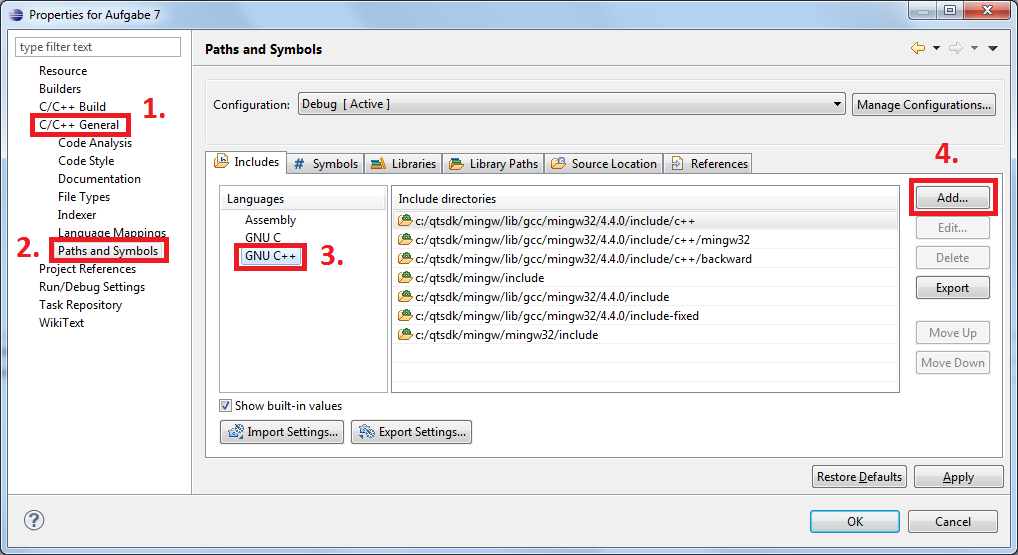
\includegraphics[width=0.94\textwidth]{boost.png}

\item Erstellen Sie eine Klasse \emph{TreeNode}, die einen Knoten eines Binärbaums darstellt. Jeder Knoten hat einen Inhalt (int) sowie einen Zeiger auf seine beiden Kindknoten. Diese Zeiger werden Smart Pointers sein, die das Speichermanagement übernehmen. Dadurch wird es nicht nötig sein, Kindknoten manuell zu löschen. Sie werden automatisch entfernt, sobald der Wurzelknoten gelöscht ist und keine Zeiger mehr auf den Kindknoten zeigen.

\begin{lstlisting}
#include <boost/shared_ptr.hpp>

class TreeNode;

// typedef for better reading
typedef boost::shared_ptr<TreeNode> TreeNodePtr;

class TreeNode {
public:
	/** Creates a new tree node and makes it shared */
	static TreeNodePtr createNode(int content, TreeNodePtr left = TreeNodePtr(), TreeNodePtr right = TreeNodePtr());

	/** Tree node destructor **/
	~TreeNode();

private:
	/** Creates a tree node */
	TreeNode(int content, TreeNodePtr left, TreeNodePtr right);

	/** left and right child */
	TreeNodePtr leftChild, rightChild;

	/** node content */
	int content;
};
\end{lstlisting}

Wie Sie sehen können, ist der Konstruktor von TreeNode privat. Dies hat folgenden Grund: sobald es Smart Pointer auf ein Objekt gibt, übernehmen diese die Verantwortung für die Lebenszeit des Objektes und bestimmen, wann es gelöscht wird. Man sollte deshalb unterlassen, Objekte von diesem Typ direkt auf dem Stack anzulegen. Andernfalls kann es passieren, dass der Objektdestruktor mehrmals aufgerufen wird, einmal vom Smart Pointer und einmal beim Verlassen der Funktion. Ebenso sollte man vermeiden, Rohzeiger auf das Objekt zu erzeugen, da diese das Speichermanagement der Smart Pointer umgehen.\\

Deshalb werden wir es nicht zulassen, dass \emph{TreeNode}-Objekte auf dem Stack erzeugt werden können. Stattdessen stellen wir eine statische Methode bereit, um \emph{TreeNode}-Objekte auf dem Heap zu erzeugen und diese direkt einem Smart Pointer zu übergeben. \\

Implementieren Sie den Konstruktor, Destruktor sowie \emph{createNode}. Der Konstruktor sollte die Attribute entsprechend initialisieren. Schreiben Sie auch eine Textausgabe, die den Zeitpunkt der Erzeugung eines \emph{TreeNode}s deutlich macht. Der Destruktor braucht die Kindknoten nicht zu löschen, da dies bei der Zerstörung des Elternknotens automatisch geschieht. Fügen Sie stattdessen auch hier eine Textausgabe ein, die die Zerstörung des Objekts sichtbar macht. \\

Das Schlüsselwort \textbf{static} sowie die Default-Parameter müssen bei der Implementierung der Methode ausgelassen werden. Der Smart Pointer für die Rückgabe wird mit einem Zeiger auf ein \emph{TreeNode}-Objekt initialisiert. Somit lautet der Methodenrumpf
\begin{lstlisting}
TreeNodePtr TreeNode::createNode(int content, TreeNodePtr left, TreeNodePtr right) {
	return TreeNodePtr(new TreeNode(...));
}
\end{lstlisting}

\item Testen Sie, ob die einzelnen Knoten tatsächlich gelöscht werden, sobald kein Zeiger mehr auf den Elternknoten zeigt. Erstellen Sie dafür mittels 
\begin{lstlisting}
TreeNodePtr node = TreeNode::createNode(1, TreeNode::createNode(2), TreeNode::createNode(3));
\end{lstlisting}

einen kleinen Baum. Führen Sie das Programm aus und beobachten Sie die Ausgabe. Sobald die \emph{main} verlassen wird, wird der Zeiger \emph{node} gelöscht, und somit auch das dahinterliegende \emph{TreeNode}-Objekt mit all seinen Kindknoten. \\

Um ganz sicher zu gehen, dass der Baum tatsächlich beim Löschen des letzten Zeigers zerstört wurde und nicht etwa durch das Beenden des Programms, können Sie \emph{node} mit einem anderen Baum überschreiben. Fügen Sie in diesem Fall am Ende des Programms eine Textausgabe hinzu, damit es ersichtlich wird, dass der erste Baum noch vor Verlassen der \emph{main} gelöscht wurde.

\item Nun wollen wir \emph{TreeNode} so erweitern, dass jeder Knoten Kenntnisse über seinen Elternknoten besitzt. Fügen Sie das Attribut  
\begin{lstlisting}
	/** parent node */
	TreeNodePtr parent;
\end{lstlisting}

hinzu. Da der Elternknoten beim Erzeugen eines \emph{TreeNode}s undefiniert ist, brauchen Sie den Konstruktor nicht zu ändern. \emph{parent} wird dann automatisch mit NULL initialisiert.\\

Implementieren Sie die Methode
\begin{lstlisting}
	/** Set parent of this node */
	void setParent(const TreeNodePtr& p);
\end{lstlisting}

um den Elternknoten zuzuweisen. Hinweis: \emph{p} wird in diesem Fall nur deshalb als const Referenz übergeben, da es verhältnismäßig aufwändig ist, einen Smart Pointer zu kopieren. Beachten Sie, dass im obigen Fall der Smart Pointer selbst const ist, und nicht das Objekt, worauf er zeigt.\\

Jetzt muss noch \emph{createNode()} modifiziert werden, sodass \emph{setParent()} auf den Kindknoten aufgerufen wird. Da ein Smart Pointer die Operatoren $*$ und $->$ überladen hat, lässt er sich syntaktisch wie ein normaler Zeiger benutzen. Um zu überprüfen, ob ein Smart Pointer auf ein Objekt zeigt, kann dieser implizit nach \emph{bool} gecastet werden. Somit lautet die neue Implementierung von \emph{createNode()}

\begin{lstlisting}
TreeNodePtr TreeNode::createNode(int content, TreeNodePtr left, TreeNodePtr right) {
	TreeNodePtr node(new TreeNode(content, left, right));
	if (left)
		left-> ... ; // set parent node
	if (right)
		right-> ... ; // set parent node
	return node;
}
\end{lstlisting}

\item
Testen Sie Ihre Implementierung. Sie brauchen dazu in der \emph{main} nichts zu ändern.\\

Wie Sie sehen, werden \emph{TreeNode}-Objekte nun überhaupt nicht gelöscht! Die Ursache dafür sind zirkuläre Abhängigkeiten in den Knoten. Denn selbst wenn Sie keine Zeiger auf den Wurzelknoten eines Baumes haben, verweisen die Kindknoten noch immer darauf. \\

Um dieses Problem zu lösen, müssen die Verweise zum Elternknoten \emph{schwach} sein. Das bedeutet, dass ein Knoten gelöscht werden darf, sobald nur noch schwache Zeiger (oder keine) auf ihn verweisen. Binden Sie dazu den Header \emph{boost/weak\_ptr.hpp} ein und erstellen Sie ein neues typedef für einen schwachen \emph{TreeNode} Smart Pointer.

\begin{lstlisting}
typedef boost::weak_ptr<TreeNode> TreeNodeWeakPtr;
\end{lstlisting}

Ändern Sie nun den Typ von parent auf \emph{TreeNodeWeakPtr} um. Es müssen keine anderen Änderungen gemacht werden da starke Zeiger (\emph{shared\_ptr}) implizit in schwache Zeiger (\emph{weak\_ptr}) umgewandelt werden können.

\item
Testen Sie Ihre Implementierung. Nun sollte sich \emph{TreeNode} wie gewünscht verhalten.

\end{enumerate}

\section{Fortsetzung Aufzug}
In dieser Aufgabe soll der Aufzug von gestern erweitert und mithilfe der neu erlernten Methoden angepasst werden, sodass das Kopieren von Personen wegfällt. Dies werden wir erreichen, in dem wir nicht mit Personen direkt sondern mit Smart Pointers auf Personen arbeiten. Dadurch müssen beim Verschieben von Personen in den Aufzug nur die Smart Pointers kopiert werden, während die \emph{Person}-Objekte selbst bestehen bleiben.

\begin{enumerate}
\item Als erstes werden wir die Sauberkeit des vorhandenen Codes mithilfe der bisher kennengelernten Mittel wie Referenzen und \emph{const} verbessern. Deklarieren Sie dafür sämtliche Getter in \emph{Building}, \emph{Elevator}, \emph{Floor} und \emph{Person}
als \emph{const}, z.B. \emph{Building::getFloor()} und \emph{Elevator::getEnergyConsumed()}. Schreiben Sie außerdem die Methode \emph{Elevator::addPeople()} so um, dass die Liste \emph{people} nicht mehr als Wert sondern als \emph{const Refernce} übergeben wird, um unnötige Kopien zu vermeiden. Hinweis: um über eine \emph{const} Liste zu iterieren, verwenden Sie \emph{vector<T>::const\_iterator} anstatt \emph{vector<T>::iterator} als Iterator-Typ.

\item Binden Sie in Ihrem Projekt den boost-Ordner in den Include-Pfad des Compilers ein.

\item Um nicht immer wieder \emph{boost::shared\_ptr<Person>} schreiben zu müssen, werden wir mittels \textbf{typedef} eine Abkürzung \emph{PersonPtr} für diesen Typen definieren. Binden Sie in \emph{Person.h} den Header \emph{boost/shared\_ptr.hpp} ein und definieren Sie den neuen Typen \emph{PersonPtr} hinter der Klassendefinition von \emph{Person} mittels

\begin{lstlisting}
typedef boost::shared_ptr<Person> PersonPtr;
\end{lstlisting}

\item Ändern Sie in der Klasse \emph{Elevator} alle Vorkommen von \emph{vector} nach \emph{list} um, da wir nun eine Verkettete Liste verwenden werden, um Personen zu speichern. Dadurch kann man Personen auch in mitten der Liste effizient löschen. \\
Sie werden feststellen, dass die list-Klasse keine Methode \emph{at()} enthält. Diese ist auch nicht nötig. Stattdessen werden wir die Liste mit einem Iterator traversieren. Löschen Sie dazu die Methode \emph{getPerson()} und fügen Sie die Methode  

\begin{lstlisting}
	/** return a const reference to list of contained people */
	const std::list<PersonPtr>& getContainedPeople() const;
\end{lstlisting}

hinzu, die eine const Referenz auf das \emph{containedPeople} Attribut zurückgibt. Dadurch kann von extern lesend auf die Leute im Aufzug zugegriffen werden. Ändern Sie außerdem den Inhaltstyp des Containers von \emph{Person} auf \emph{PersonPtr}, da wir Smart Pointer auf Personen speichern werden und nicht die Personen direkt. Passen Sie die Signaturen aller Methoden in \emph{Elevator} entsprechend an. \\

\item
Jetzt müssen wir die Methode \emph{removeArrivedPeople()} anpassen. Da wir beliebige Elemente aus \emph{containedPeople} löschen können, brauchen wir den Umweg über den temporären \emph{stay} Vector nicht mehr. \\

Gehen Sie dazu folgendermaßen vor: Legen Sie einen Listeniterator vom Typ \textbf{std::list<PersonPtr>::iterator} an und initialisieren Sie ihn mit dem Anfang der Liste (\emph{containedPeople.begin()}). Solange der Iterator ungleich \emph{containedPeople.end()} ist, prüfen  Sie, ob die Person, auf die der Iterator zeigt, an ihrem Ziel angekommen ist. Sie können das Element, auf den der Iterator zeigt, durch den Dereferenzierungsoperator (\emph{*iter}) holen. Beachten Sie, dass dieses Element selbst ein Smart Pointer ist und deshalb zum Zugriff nochmal dereferenziert werden muss. Wenn die Person in ihrem Zielstockwerk angekommen ist, wird sie aus \emph{containedPeople} gelöscht zu \emph{arrived} hinzugefügt. Um ein Element zu löschen, verwenden Sie \emph{containedPeople.erase(iter)}. Die Methode wird Ihnen den Iterator auf das nächste Element der Liste zurückgeben.\\

Als Grundgerüst kann Ihnen folgendes Codeschnipsel dienen:

\begin{lstlisting}
	// create iterator for containedPeople
	... iter = containedPeople. ...;
	
	// iterate through all elements
	while (iter != ...) {
		PersonPtr person = ... iter; // get person smart pointer at current position
		
		// check whether person has reached it's destination Floor
		if (...) {
			// erase person pointer from containedPeople
			// no need for ++iter since iter will already point to next item
			... = containedPeople.erase(iter);
			
			// remember arrived person 
			...
		} else
			++iter; // check next person
	}
\end{lstlisting}

\item Passen Sie auch die Klassen \emph{Floor} und \emph{Building} entsprechend an, sodass nur noch Listen und Smart Pointer auf Personen verwendet werden.

\item
Passen Sie die Simulation des Aufzugs entsprechend an. Sie werden auf die erste Person im Aufzug nun auf eine andere Art und Weise zugreifen müssen als vorher. Benutzen Sie die Methode \emph{getContainedPeople()} des Aufzugs, um an die Liste der Personen zu kommen. Nun können Sie auf den Inhalt des ersten Elements mittels \emph{front()} zugreifen. Vergessen Sie nicht, dass dieser Inhalt ein Smart Pointer auf eine Person und nicht die Person direkt ist. Deshalb müssen Sie einen anderen Operator als $.$ verwenden, um auf die Methoden der Person zuzugreifen. \\

Schauen Sie sich die Ausgabe an. Nun werden Personen nicht mehr kopiert, sondern nur noch gelöscht, sobald sie tatsächlich den Aufzug verlassen haben und kein Zeiger mehr auf sie zeigt.

\end{enumerate}

\end{document}
